\section{RAVEN Concepts}
\label{sec:RAVENconcept}
After the brief overview of the RAVEN code, it is necessary to focus on the main concepts that are behind the design of the framework:
\begin{itemize}
    \item \textit{Mathematical Background}: Section ~\ref{sub:mathBackground} provides an description of the mathematical background of RAVEN,
     overall focalizing on the probabilistic dynamics
    \item \textit{RAVEN entities}: Section ~\ref{sub:EntitiesAndFlow} is aimed to provide an overview on how the different objects in
    RAVEN can interact with each other, generating the user-dependent analysis flow
    \item \textit{RAVEN input main components}: Section ~\ref{sub:InputStructure} provides a brief introduction of the input structure, introducing
    some of the input ``structure'' that are going to be used in this manual. A detailed explanation of the
    input structure and keywords is reported in the user manual ~\cite{RAVENuserManual}.
\end{itemize}
\subsection{RAVEN Mathematical Background}
\label{sub:mathBackground}
\subsubsection{System and Control Model}
\label{subsub:controlAndSystem}
The first step is the derivation of the mathematical model representing, with a high
level of abstraction, the plant and control system model. Let $\overline{\theta}\left ( t
\right )$ be a vector describing the system status in the phase space, characterized
by the following governing equation:
\begin{equation}
\label{eq:dThetaOverDT}
\frac{\partial \overline{\theta} }{\partial t}=\overline{H}\left (  \overline{\theta}\left ( t \right ),t \right )
\end{equation}
In Equation above, the assumption of time differentiability of the trajectory equation $\overline{H}\left (  \overline{\theta}\left ( t \right ),t \right )$ in the phase space has been taken. This assumption is not fully correct and generally required and it is used here, without missing of generality, for compactness of the notation.
\\It can now be performed an arbitrary decomposition of the phase space:
\begin{equation}
\label{eq:thetaDecomposition}
  \overline{\theta} = \left (\frac{\overline{x}}{\overline{v}}  \right )
\end{equation}
The decomposition is made in such a way that $\overline{x}$ represent the unknowns
solved by a system code (such as RELAP5-3D~\cite{RELAP5userManual},
RELAP7~\cite{relap7FY12}, etc.) while $\overline{v}$ are the variables directly
controlled by the control system (e.g., automatic mitigation systems, operator actions,
etc.).
\\The governing equation can be now cast in the following system of equations:
\begin{equation}
\label{eq:governingEquations}
\left\{\begin{matrix}
\frac{\partial \overline{x} }{\partial t} = \overline{F}\left (  \overline{x}, \overline{v}, t \right )  \\
\frac{\partial \overline{v} }{\partial t} = \overline{V}\left (  \overline{x}, \overline{v}, t \right )
\end{matrix}\right.
\end{equation}
Consequentially to this splitting, $\overline{x}$ contains the state variables of the
phase space that are continuous while $\overline{v}$ contains discrete state
variables that are usually handled by the control system (consequentially, named
\textbf{control variables}). It can be noticed that the
function  $ \overline{V}\left (  \overline{x}, \overline{v}, t \right )$, representing the
control system, does not depend on the  knowledge of the complete status of the
system but on a restricted subset that can be named \textbf{monitored variables} $\overline{C}$:

\begin{equation}
\label{eq:controlVars}
\left\{\begin{matrix}
\frac{\partial \overline{x} }{\partial t} = \overline{F}\left (  \overline{x}, \overline{v}, t \right )  \\
 \overline{C} =  \overline{G}(\overline{x},t)     \\
\frac{\partial \overline{v} }{\partial t} = \overline{V}\left (  \overline{x}, \overline{v}, t \right )
\end{matrix}\right.
\end{equation}
where $\overline{C}$ is a vector of smaller dimensionality than $\overline{x}$ and,
therefore, more convenient to handle.
\\As it can be noticed, the standard nomenclature of \textit{signals} (monitored variables) and \textit{status} (control variables) is not adopted. Two principal reasons
justify this decision:
\begin{itemize}
  \item The definition of signals is tight to the definition of the
  control logic for each component and, therefore, relative rather than absolute in the
  overall system analysis. For example, it is possible the the \textit{signals} for a
  component represent \textit{status} of another one, determining an in-unique
  definition.
  \item The standard nomenclature becomes meaningless when this derivation is
  applied to Uncertainty Quantification (UQ).
\end{itemize}

\paragraph{Splitting Approach for the Simulation of the Control System}
Equation~\ref{eq:controlVars} represents a fully coupled system of Partial Differential
Equations (PDEs). To solve this system, an  \textit{operator splitting} approach
is employed. This method is preferable in this context for several reasons, among which the following:
\begin{itemize}
  \item In reality, the control system (automatic mitigation systems, operator actions,
  etc.) is always characterized by an intrinsic delay
  \item The reaction of the control system might make the system ``move'' among
  different discrete states; therefore, numerical errors will be always of first order
  unless the discontinuity is explicitly treated.
\end{itemize}
Employing the \textit{operator splitting} approach, Equation ~\ref{eq:controlVars}  can be
cast as follows:
\begin{equation}
\label{eq:operatorSplitting}
\left\{\begin{matrix}
\frac{\partial \overline{x} }{\partial t} = \overline{F}\left (  \overline{x},\overline{v}_{t_{i-1}}, t \right )  & \\
\overline{C} =  \overline{G}(\overline{x},t)  & t_{i-1} \leq t \leq  t_{i} =  t_{i-1} + \Delta  t_{i}\\
\frac{\partial \overline{v} }{\partial t} = \overline{V}\left (  \overline{x}, \overline{v}_{t_{i-1}}, t \right ) &
\end{matrix}\right.
\end{equation}
Hence, the system of equations in solved decomposing it into simpler sub-problems that are treated individually
using specialized numerical algorithms.

\paragraph{Definition of the Monitored Variable Space}
The contraction of the information from the $\overline{x}$ space to the $\overline{C}$ space is a crucial step.
Since $\overline{C}$ represents an arbitrary middle step, it is needed to define a set of rules that make this
choice unique. $\overline{C}$ is chosen such that:
\begin{itemize}
  \item The solution of  $ \left.\begin{matrix} \frac{\partial \overline{v} }{\partial t}
  \end{matrix}\right| =\overline{V}\left (  \overline{x},\overline{v}_{t_{i-1}}, t \right )$
  can be carried along without any knowledge of the solution algorithm of
   $ \left.\begin{matrix}
  \frac{\partial \overline{x} }{\partial t} =  \end{matrix}\right| \overline{F}\left (
  \overline{x},\overline{v}_{t_{i-1}}, t \right )
  $. This requirement determines the minimum information contraction from  $\overline{x}$ to
  $\overline{C}$.
  \item All actions represented by $\overline{C} = \overline{G}(\overline{x},t)$ require knowledge of the
  solution algorithm of
  $ \left.\begin{matrix}
  \frac{\partial \overline{x} }{\partial t} =  \end{matrix}\right| \overline{F}\left (
  \overline{x},\overline{v}_{t_{i-1}}, t \right )  $. This requirement determines  the maximum  information contraction from  $\overline{x}$ to  $\overline{C}$.
\end{itemize}
The intersection of the two sub-spaces defined above create a minimal unique set.
\paragraph{Definition of the Auxiliary Variable Space}
In the previous sections, it has been determined that the needed information to model the dynamic system
is contained in the solution vectors $\overline{x}$ and $\overline{v}$. Even if $\overline{x}$ and $\overline{v}$
are sufficient to assess the system status at every point in time, it can result in an unpractical way to model
the eventual control system.
Let's suppose to model a component of a particular system that presents different behavior depending on
other systems or operation behaviors. In order to define the status of this component in every point in time, the
whole history of the system needs to be tracked. In order to remove these inefficiency, a set of auxiliary variables
$\overline{a}$ can be introduced. These variables are the ones that in the analysis of stochastic dynamics
are artificially added into the phase space to a non-Markovian system to obtain back a Markovian behavior. In this
way only the previous time-step information is needed to determine the status of the system.
\\ Adding this additional system of variables, Equation ~\ref{eq:operatorSplitting} can be casted as follows:

\begin{equation}
\label{eq:auxiliaryVariables}
\left\{\begin{matrix}
\frac{\partial \overline{x} }{\partial t} = \overline{F}\left (  \overline{x},\overline{v}_{t_{i-1}}, t \right )  & \\
\overline{C} =  \overline{G}(\overline{x},t)  & t_{i-1} \leq t \leq  t_{i} =  t_{i-1} + \Delta  t_{i}\: \\
\frac{\partial \overline{a} }{\partial t} = \overline{A}\left (  \overline{x},\overline{C},\overline{a},\overline{v}_{t_{i-1}}, t \right ) \\
\frac{\partial \overline{v} }{\partial t} = \overline{V}\left (  \overline{C},\overline{a}, \overline{v}_{t_{i-1}}, t \right )  &
\end{matrix}\right.
\end{equation}

\subsubsection{Dynamic Systems Stochastic Modeling}
%
\paragraph{General system of equations and variable classification}
\label{par:generalSystemOfEqAndVarsClassification}
In Section ~\ref{subsub:controlAndSystem}, the derivation of the governing equations for a controllable system
have been reported. In this section, the mathematical framework of the modeling of dynamic stochastic systems,
under uncertainties, is derived.
\\ Dynamic stochastic systems are the ones whose dynamic is characterized by intrinsic randomness. Random
behaviors, although present in nature, are often artificially introduced into physical models to account for the
incapability of fully modeling part of the nature of the system behavior and/or of the phenomena bounding the
physical problem.
\\The distinction between variables that are artificially considered aleatory and the ones intrinsically aleatory
corresponds with the classical definition of epistemic and aleatory uncertainties. From a
system simulation point of view it is more relevant how these variables, the sources of aleatory behavior, change
in time.
Possible examples of random elements are:
\begin{itemize}
 \item random variability of parameters (e.g., uncertainty in physical parameters)
 \item presence of noise (background noise due to intrinsically stochastic behaviors or lack of detail in the
 simulation)
 \item Uncertainty in the initial and boundary conditions
 \item Random failure of components
 \item aging effects.
\end{itemize}
Before introducing the mathematical models for uncertainty,  it can beneficial to recall
Equation ~\ref{eq:dThetaOverDT}, adding the initial conditions:
\begin{equation}
\label{eq:dThetaOverDTWithBoundary}
\left\{\begin{matrix}
\frac{\partial  \overline{\theta}\left ( t \right )}{\partial t}=\overline{H}\left (  \overline{\theta}\left ( t \right ),t \right ) \\
 \overline{\theta}\left ( t_{0} \right ) = \overline{\theta}_{0}
\end{matrix}\right.
\end{equation}
At this point, each source of uncertainty or stochastic behavior is considered and progressively added in
Equation ~\ref{eq:dThetaOverDTWithBoundary}.
For the scope of this derivation, it is convenient to split the phase space into \textit{continuous} (e.g.,temperature,
pressure, hentalpy, etc.) and discrete (e.g.,status of components, such as operational and failure states) variables
as follows:
\begin{itemize}
 \item $ \overline{\theta}^{c} \in \Phi \subseteq \mathbb{R}^{C}$, the set of continuous variables
 \item $ \overline{\theta}^{d} \in \Psi \subseteq \mathbb{N}^{D}$, the set of discrete variables
 \item $\overline{\theta}(t) = \overline{\theta}^{c} \oplus \overline{\theta}^{d}$.
\end{itemize}
Consequentially, Equation ~\ref{eq:dThetaOverDTWithBoundary} assumes the following form:
\begin{equation}
\label{eq:systemThetaContAndDescrete}
\left\{\begin{matrix}
\frac{\partial  \overline{\theta}^{c}\left ( t \right )}{\partial t}=f\left ( \overline{\theta}^{c},\overline{\theta}^{d},t \right ) \\
\frac{\partial  \overline{\theta}^{d}\left ( t \right )}{\partial t}=g\left ( \overline{\theta}^{c},\overline{\theta}^{d},t \right )\\
 \overline{\theta}^{c}\left ( t_{0} \right ) = \overline{\theta}^{c}_{0}\\
 \overline{\theta}^{d}\left ( t_{0} \right ) = \overline{\theta}^{d}_{0}
\end{matrix}\right.
\end{equation}
Note that the time derivative operator has been also used for the time discontinuous variables, even
if this is allowed only introducing complex extension of the time derivative operator. In this context, the $\frac{\partial  }{\partial t}$ on the discontinuous space is employed for simplifying the notation only.

\paragraph{Probabilistic Nature of the Parameters Characterizing the Equation}
As shown in Equation ~\ref{eq:systemThetaContAndDescreteStaz}, The first stochastic behaviors to be introduced are the
uncertainties associated with the:
\begin{itemize}
  \item initial conditions (i.e. $\overline{\theta}^{c}$ and $\overline{\theta}^{d}$ at time $t_{0}$), and
  \item parameters characteristic of  $f\left ( \overline{\theta}^{c},\overline{\theta}^{d},t \right )$ and $g\left ( \overline{\theta}^{c},\overline{\theta}^{d},t \right )$.
\end{itemize}

\begin{equation}
\label{eq:systemThetaContAndDescreteStaz}
\left\{\begin{matrix}
\frac{\partial  \overline{\theta}^{c}\left ( t \right )}{\partial t}=f\left ( \overline{\theta}^{c},\overline{\theta}^{d}, \overline{\alpha}_{staz} ,      t \right ) \\
\frac{\partial  \overline{\theta}^{d}\left ( t \right )}{\partial t}=g\left ( \overline{\theta}^{c},\overline{\theta}^{d},\overline{\alpha}_{staz},t \right )\\
\Pi \left ( \overline{\theta}^{c},t_{0} \right ) \sim pdf\left ( \overline{\theta}^{c}_{0}|,\sigma_{c}^{2} \right )\\
\Pi \left ( \overline{\theta}^{d},t_{0} \right ) \sim pdf\left ( \overline{\theta}^{d}_{0}|,\sigma_{d}^{2} \right ) \\
\overline{\alpha}_{staz}\left ( t \right )=\overline{\alpha}_{staz}\left ( t_{0} \right ) \sim pdf\left ( \overline{\alpha}_{staz}^{0}|, \sigma_{staz}^{2} \right )
\end{matrix}\right.
\end{equation}
In Equation ~\ref{eq:systemThetaContAndDescreteStaz}, $\Pi \left ( \overline{\theta}^{c},t_{0} \right )$ indicates the
probability distribution of $\overline{\theta}^{c}$ at the initial time $t=t_{0}$ while
$pdf\left ( \mu|, \sigma^{2} \right )$ represents a generic probability distribution function having mean value
$\mu$ and sigma $\sigma$.The term $\overline{\alpha}_{staz}$ is the vector of parameters affected by
uncertainty but not varying over time.
\\As already mentioned, Equation ~\ref{eq:systemThetaContAndDescreteStaz} considers uncertainties whose values
do not change during the dynamic evolution of the system. This set of uncertainties accounts for most of the
common source of aleatory behaviors. Examples of this kind of uncertainties are:
\begin{itemize}
  \item \textit{Uncertainty associated with the heat conduction coefficient}:  This value is known (but uncertain) and has no physical reason to change during the simulation;
  \item \textit{Uncertainty on failure temperature for a pipe}: This value is usually characterized by a probability distribution function but once the value has been set (like through random sampling) it will not change during the simulation.
\end{itemize}
From a modeling perspective, all the probabilistic behaviors connected to $\Pi \left ( \overline{\theta}^{c},t_{0}
\right ) $, $\Pi \left ( \overline{\theta}^{d},t_{0} \right )$ and $\overline{\alpha}_{staz}(t)$ can be modeled without
changing the dimensionality of the phase space (hence, no alteration of the solution algorithm is required), simply performing sampling of the input space. In addition, the Markovian assumption is still preserved.

\paragraph{Variables Subject to Random Motion}
The next aleatory component to be accounted for is the set of parameters that continuously change over time (i.e. $\overline{\alpha}_{brow}$).
In other words,  these parameters are referred as if they behave like a \textit{Brownian motion}.
While what commonly is indicated as \textit{Brownian motion} has not impact at the character
the space and time scales (characteristic of a physical system), there are parameters that have (or \textbf{appear}
to have) such behavior. The  \textit{Brownian motion} characteristic of some variables can be completely
synthetic, due to the lack of modeling details in the simulation model.
\\For instance, two examples of these randomly varying variables are:
\begin{itemize}
  \item \textit{Cumulative damage growth in material}. Experimental data and models representing this
  phenomenon show large uncertainties. There is also an intrinsic natural stochasticity driving
  the accumulation of the damage (natural Brownian motion);
  \item \textit{Heat conductivity in the fuel gap during heating of fuel}. During some transients there are
  situations where the fuel is in contact with the clad while in others where there is the presence of a gap. While in
  nature this is a discontinuous transition, it is not usually possible to model in such a way, especially if vibrations
  of the fuel lead to high frequency oscillations. In this case, it would be helpful to introduce directly into the
  simulation a random noise characterizing the thermal conductivity when these transitions occur (synthetic
  Brownian motion).
\end{itemize}
The system of Equations~\ref{eq:systemThetaContAndDescreteStaz} can be rewritten in the following form:

\begin{equation}
\label{eq:systemThetaContAndDescreteStazAndBrow}
\left\{\begin{matrix}
\frac{\partial  \overline{\theta}^{c}\left ( t \right )}{\partial t}=f\left ( \overline{\theta}^{c},\overline{\theta}^{d}, \overline{\alpha}_{staz} ,\overline{\alpha}_{brow},      t \right ) \\
\frac{\partial  \overline{\theta}^{d}\left ( t \right )}{\partial t}=g\left ( \overline{\theta}^{c},\overline{\theta}^{d},\overline{\alpha}_{staz},\overline{\alpha}_{brow},t \right )\\
\frac{\partial \overline{\alpha}_{brow} }{\partial t}=b\left ( \overline{\theta}^{c},\overline{\theta}^{d},\overline{\alpha}_{staz},\overline{\alpha}_{brow},t \right )\Gamma \left ( t \right )
\\
\Pi \left ( \overline{\theta}^{c},t_{0} \right ) \sim pdf\left ( \overline{\theta}^{c}_{0}|,\sigma_{c}^{2} \right )\\
\Pi \left ( \overline{\theta}^{d},t_{0} \right ) \sim pdf\left ( \overline{\theta}^{d}_{0}|,\sigma_{d}^{2} \right ) \\
\overline{\alpha}_{staz}\left ( t \right )=\overline{\alpha}_{staz}\left ( t_{0} \right ) \sim pdf\left ( \overline{\alpha}_{staz}^{0}|, \sigma_{staz}^{2} \right ) \\
\overline{\alpha}_{brow}\left ( t_{0} \right ) \sim  \overline{\alpha}_{brow}^{0} \Gamma \left ( t_{0} \right )
\end{matrix}\right.
\end{equation}
where $\Gamma \left ( t \right )$ is 0-mean random noise and $\overline{\alpha}_{brow}$ is the set of parameters subject to \textit{Brownian motion}.
\\Clearly, the equation referring to the time change of the parameters subject to the \textit{Brownian motion} should be interpreted in the \textbf{Ito} sense [C. Gardiner, Stochastic Methods, Springer (2009)].

\paragraph{Discontinuously and Stochastically varying variables}
The last and probably most difficult step is the introduction of parameters that are neither constant during the simulation nor continuously vary over time. As an example, consider a valve that, provided set of operating conditions, opens or closes. If this set of conditions is reached n times during the simulation, the probability of the valve correctly operating should be sampled n times. It is also foreseeable that the history of failure/success of the valve will impact future probability of failure/success.  In this case the time evolution of such parameters (discontinuously stochastic changing parameters  $\overline{\alpha}_{DS}$) is governed by the following equation:

\begin{equation}
\label{eq:systemDiscAndStochVaryVars}
\frac{\partial  \overline{\alpha }_{DS}\left ( t \right )}{\partial t}=  \overline{\delta}\left ( \overline{\alpha }_{DS}, \overline{\theta}^{c},\overline{\theta}^{d},\overline{\alpha}_{staz},\overline{\alpha}_{brow},t \right ) \times \overline{V}\left ( \overline{\alpha }_{DS}, \overline{\theta}^{c},\overline{\theta}^{d},\overline{\alpha}_{staz},\overline{\alpha}_{brow},t \right ) \times \overline{p}\left ( \int_{t_{0}}^{t}  S\left ( \overline{\theta}\left ( t^{'} \right ),t^{'} \right )dt^{'} \right )
\end{equation}
where:
\begin{itemize}
  \item The function $\overline{\delta}\left ( \overline{\alpha }_{DS}, \overline{\theta}^{c},\overline{\theta}^{d},
  \overline{\alpha}_{staz},\overline{\alpha}_{brow},t \right )$ is the delta of Dirac of the instant on which the
  transition need to be evaluated (control logic signaling to the valve to open/close).
  \item The term $\overline{p}\left ( \int_{t_{0}}^{t}  S\left ( \overline{\theta}\left ( t^{'} \right ),t^{'} \right )\right )
  = \overline{p}\left ( \int_{t_{0}}^{t}  \overline{\alpha }_{DS}, \overline{\theta}^{c},\overline{\theta}^{d},
  \overline{\alpha}_{staz},\overline{\alpha}_{brow},t dt\right )$ represents the transition probability
  between different states (in case of the valve: open/close). Note that the time integral of the
  parameter history accounts for the memory of the component via the kernel $S\left ( \overline{\theta}\left ( t^{'}
  \right ),t^{'} \right )$.
  \item The term $\overline{V}\left ( \overline{\alpha }_{DS}, \overline{\theta}^{c},\overline{\theta}^{d},
  \overline{\alpha}_{staz},\overline{\alpha}_{brow},t \right )$ is the rate of change of $\overline{\alpha }_{DS}$.
  For a discrete parameter, it is defined as the value of the instantaneous $\overline{\alpha }_{DS}$ change.
\end{itemize}
The introduction of the history dependency introduced in the term $\overline{p}$ determines that the system cannot be considered
Markovian if ``countermeasures'' are not taken. In order to make the system return to be Markovian, the phase space needs to be
expanded (i.e., increase its dimensionality): the time at which the
parameters changed status and their corresponding values $\left \{  \left (\overline{\alpha}_{DS}, t \right )_{i} \right \} = \left \{  \overline{\alpha}_{DS}, t_{i} \right \} = \overline{\overline{\alpha}}_{DS}, \overline{t}\, \left ( for\, i=1,...,n \right )$.
\\Equation~\ref{eq:systemDiscAndStochVaryVars} now assumes the form:
\begin{equation}
\label{eq:systemDiscAndStochVaryVarsExpanded}
\begin{matrix}
\frac{\partial  \overline{\alpha }_{DS}\left ( t \right )}{\partial t}=  \overline{\delta}\left ( \overline{\alpha }_{DS}, \overline{\theta}^{c},\overline{\theta}^{d},\overline{\alpha}_{staz},\overline{\alpha}_{brow},t \right ) \times \overline{V}\left ( \overline{\alpha }_{DS}, \overline{\theta}^{c},\overline{\theta}^{d},\overline{\alpha}_{staz},\overline{\alpha}_{brow},t \right ) \times \overline{p}\left ( \overline{\overline{\alpha}}_{DS},\overline{t},\overline{\theta}^{c},\overline{\theta}^{d},\overline{\alpha}_{staz},\overline{\alpha}_{brow},t  \right ) \\ \! \! \! \! \! \! \! \! \! \! \! \! \! \! \! \! \! \! \! \! \! \! \! \! \! \! \! \! \! \! \! \! \! \! \! \! \! \! \! \! \! \! \! \! \! \! \! \! \! \! \! \! \! \! \! \! \! \! \! \! \! \! \! \! \! \! \! \! \! \! \! \! \! \! \! \! \! \! \! \! \! \! \! \! \! \! \! \! \! \! \! \! \! \! \! \! \! \! \! \! \! \! \! \! \! \! \! \! \! \! \! \! \! \! \! \! \! \! \! \! \! \! \! \! \! \! \! \! \! \! \! \! \! \! \! \! \! \! \! \! \! \! \! \! \! \! \! \! \! \! \! \! \! \! \! \! \! \! \! \! \! \! \! \! \! \! \! \!
for \, t\geq t_{n}
\end{matrix}
\end{equation}
This formulation introduces a phase space that is continuously growing over time $n \rightarrow \infty$. In this respect, it is useful to introduce and discuss possible assumptions:
\begin{enumerate}
  \item The memory of the past is not affected by the time distance; in this case:
  \begin{equation}
   \overline{p}\left ( \overline{\overline{\alpha}}_{DS},\overline{t},\overline{\theta}^{c},\overline{\theta}^{d},\overline{\alpha}_{staz},\overline{\alpha}_{brow},t  \right ) =  \overline{p}\left ( \overline{\overline{\alpha}}_{DS},\overline{\theta}^{c},\overline{\theta}^{d},\overline{\alpha}_{staz},\overline{\alpha}_{brow},t  \right )
  \end{equation}
  The dimensionality of the phase space is still growing during the simulation since more and more sampling is
  performed, but the time integral is removed from the transition probability. A simple example of this situation is
  a component activated on demand in which failure is a function of all previous sampling, but not of when the
  component was sampled or in which sequence the outcome occurred.
  \item  The number of samples is determined before the simulation itself takes place (e.g.,$n$ times) In this case
  the different $\overline{\alpha}_{DS_{i}}$ could be treated explicitly as $\overline{\alpha}_{staz}$   while
  $\overline{t}$ would still remain a variable to be added to the phase space (if simplification 1 is not valid) but of
  fixed dimension. In this case $\overline{t}$ still needs to be computed and its expression is:
  \begin{equation}
   \overline{t} \left ( t \right ) = \int_{t_{0}}^{t} \overline{t}  \, \overline{\delta }\left ( \overline{\alpha }_{DS},
   \overline{\theta}^{c},\overline{\theta}^{d},\overline{\alpha}_{staz},\overline{\alpha}_{brow},t \right )  dt
  \end{equation}
  The transition probability becomes:
  \begin{equation}
     \overline{p}\left ( \int_{t_{0}}^{t} dt\, S\left ( \overline{t} \right ), \overline{\alpha}_{DS}, \overline{\theta}^{c},
     \overline{\theta}^{d},\overline{\alpha}_{staz},\overline{\alpha}_{brow},t \right )
  \end{equation}
  For example, this is the case of a component that is sampled a fixed number of times for a given simulation
  while the contribution of the history to the transition probability might decay exponentially over time. This
  approximation might eliminate the memory from the system by adding n variables to the phase space $t_{i} \, \,
  (for \, \, i=1,...,n)$ thus restoring the Markovian characteristic.
  \item Another possible approximation alternative to the previous one is that the memory of the system (here
  explicitly represented by $ \int_{t_{0}}^{t}  \overline{\alpha }_{DS} dt$) is limited
  only to a fixed number of steps back in the past. In this case $n$ is always bounded. Therefore, adding  $\left \{
  \overline{\alpha}_{DS_{i}},t_{i} \right \}, \left ( for\: i=1,...,n \right )$ would possibly preserve the system
  Markovian properties of the system. This approximation allows for eliminating the memory from the system by
  expanding the phase space $2n$ variables. From a software implementation point of view, this is the most
  complex  situation since without any simplification we would have to deal with a system that is never reducible
  to a Markovian one and therefore forced to use the whole history of the system to forecast its evolution at each
  time step.
\end{enumerate}
Assumption 1 limits this cost by restraining it to the set of values assumed by the
variable but would still lead to very difficult to deal with situation. Assumption 2 would
require an expansion of phase space to introduce the time at which the transitions
happens but the value that the parameter will assume at each sampling could be
treated as initial condition. Assumption 3 would instead require the expansion of the
phase space for both the time and the values of the
transitioning variables.
\\Based on the this simplifications, the system of
Equations~\ref{eq:systemThetaContAndDescreteStazAndBrow}, accounting also for $ \overline{\alpha}_{DS}$ can be cast into the form:
\begin{equation}
\label{eq:fullSystem}
\begin{split}
\left\{\begin{matrix}
\frac{\partial  \overline{\theta}^{c}\left ( t \right )}{\partial t}=f\left ( \overline{\theta}^{c},\overline{\theta}^{d}, \overline{\alpha}_{staz} ,\overline{\alpha}_{brow},      t \right ) \\
\frac{\partial  \overline{\theta}^{d}\left ( t \right )}{\partial t}=g\left ( \overline{\theta}^{c},\overline{\theta}^{d},\overline{\alpha}_{staz},\overline{\alpha}_{brow},t \right )\\
\frac{\partial \overline{\alpha}_{brow} }{\partial t}=b\left ( \overline{\theta}^{c},\overline{\theta}^{d},\overline{\alpha}_{staz},\overline{\alpha}_{brow},t \right )\Gamma \left ( t \right ) \\
\frac{\partial  \overline{\alpha }_{DS}\left ( t \right )}{\partial t}=  \overline{\delta}\left ( \overline{\alpha }_{DS}, \overline{\theta}^{c},\overline{\theta}^{d},\overline{\alpha}_{staz},\overline{\alpha}_{brow},t \right ) \times \overline{V}\left ( \overline{\alpha }_{DS}, \overline{\theta}^{c},\overline{\theta}^{d},\overline{\alpha}_{staz},\overline{\alpha}_{brow},t \right ) \times
\\ \times  \overline{p}\left ( \int_{t_{0}}^{t}  dt\;   \overline{\alpha }_{DS}, \overline{\theta}^{c},\overline{\theta}^{d},
  \overline{ \alpha}_{staz},\overline{\alpha}_{brow},t \right )
\\
\Pi \left ( \overline{\theta}^{c},t_{0} \right ) \sim pdf\left ( \overline{\theta}^{c}_{0}|,\sigma_{c}^{2} \right )\\
\Pi \left ( \overline{\theta}^{d},t_{0} \right ) \sim pdf\left ( \overline{\theta}^{d}_{0}|,\sigma_{d}^{2} \right ) \\
\overline{\alpha}_{staz}\left ( t \right )=\overline{\alpha}_{staz}\left ( t_{0} \right ) \sim pdf\left ( \overline{\alpha}_{staz}^{0}|, \sigma_{staz}^{2} \right ) \\
\overline{\alpha}_{brow}\left ( t_{0} \right ) \sim  \overline{\alpha}_{brow}^{0} \Gamma \left ( t_{0} \right ) \\
\overline{\alpha}_{DS} \left ( t_{0} \right ) = \overline{\alpha}_{DS} ^{0}
\end{matrix}\right.
\end{split}
\end{equation}
Introducing the Simplifications \textbf{1} and \textbf{3} ( the most
appropriated in this context), Equation ~\ref{eq:fullSystem} becomes:
\begin{equation}
\label{eq:fullSystemApprox1-3}
\begin{split}
\left\{\begin{matrix}
\frac{\partial  \overline{\theta}^{c}\left ( t \right )}{\partial t}=f\left ( \overline{\theta}^{c},\overline{\theta}^{d}, \overline{\alpha}_{staz} ,\overline{\alpha}_{brow},      t \right ) \\
\frac{\partial  \overline{\theta}^{d}\left ( t \right )}{\partial t}=g\left ( \overline{\theta}^{c},\overline{\theta}^{d},\overline{\alpha}_{staz},\overline{\alpha}_{brow},t \right )\\
\frac{\partial \overline{\alpha}_{brow} }{\partial t}=b\left ( \overline{\theta}^{c},\overline{\theta}^{d},\overline{\alpha}_{staz},\overline{\alpha}_{brow},t \right )\Gamma \left ( t \right ) \\
\frac{\partial  \overline{\alpha }_{DS}\left ( t \right )}{\partial t}=  \overline{\delta}\left ( \overline{\alpha }_{DS}, \overline{\theta}^{c},\overline{\theta}^{d},\overline{\alpha}_{staz},\overline{\alpha}_{brow},t \right ) \times \overline{V}\left ( \overline{\alpha }_{DS}, \overline{\theta}^{c},\overline{\theta}^{d},\overline{\alpha}_{staz},\overline{\alpha}_{brow},t \right ) \times
\\ \times  \overline{p}\left ( \overline{\alpha }_{DS}, \overline{\theta}^{c},\overline{\theta}^{d},\overline{\alpha}_{staz},\overline{\alpha}_{brow},t \right )
\\
\Pi \left ( \overline{\theta}^{c},t_{0} \right ) \sim pdf\left ( \overline{\theta}^{c}_{0}|,\sigma_{c}^{2} \right )\\
\Pi \left ( \overline{\theta}^{d},t_{0} \right ) \sim pdf\left ( \overline{\theta}^{d}_{0}|,\sigma_{d}^{2} \right ) \\
\overline{\alpha}_{staz}\left ( t \right )=\overline{\alpha}_{staz}\left ( t_{0} \right ) \sim pdf\left ( \overline{\alpha}_{staz}^{0}|, \sigma_{staz}^{2} \right ) \\
\overline{\alpha}_{brow}\left ( t_{0} \right ) \sim  \overline{\alpha}_{brow}^{0} \Gamma \left ( t_{0} \right ) \\
\overline{\alpha}_{DS} \left ( t_{0} \right ) = \overline{\alpha}_{DS} ^{0}
\end{matrix}\right.
\end{split}
\end{equation}
This dissertation does not cover all the possible phenomena, but it
provides a sufficient mathematical framework for extrapolating toward cases that are not explicitly treated.
\\ Given the presence of all these sources of stochastic behaviors, every
exploration of the uncertainties (through sampling strategies) only
represents a possible trajectory of the system in the phase space. Hence,
it is much more informative the assessment of the probability of a
particular response, rather than the response itself.
\\The explanation of these concepts is demanded to next section.
%
%
% Formulation of the equation set in a statistical framework
%
%
\subsubsection{Formulation of the equation set in a statistical framework}
Based on the premises reported in the previous sections and assuming
that at least one of the simplifications mentioned in
Section~\ref{par:generalSystemOfEqAndVarsClassification} is applicable (i.e. the system can be
casted as Markovian), it is needed to investigate the system evolution
in terms of its probability density function in the global phase space
$\overline{\theta}$ via the Chapman-Kolmogorov
equation~\cite{ProbReactoDynamicsDevooght}.
\\The integral form of the Chapman-Kolmogorov is the following:
\begin{equation}
\label{eq:chapKolmogIntegralForm}
\begin{matrix}
\Pi \left (\overline{\theta}_{3},t_{3}|\overline{\theta}_{1},t_{1}  \right ) = \int
d\overline{\theta}_{2} \Pi\left (\overline{\theta}_{2},t_{2}|
\overline{\theta}_{1},t_{1}  \right )   \Pi\left (\overline{\theta}_{3},t_{3}|
\overline{\theta}_{2},t_{2}  \right )   &
where \: \:   t_{1} < t_{2} < t_{3}
\end{matrix}
\end{equation}
while its differential form is:
\begin{equation}
\label{eq:chapKolmogDiffForm}
\frac{\partial \Pi \left (\overline{\theta},t|\overline{\theta}_{0},t_{0}  \right )  }{\partial t} =
\mathcal{L}_{CK}\left (   \Pi \left (\overline{\theta},t|\overline{\theta}_{0},t_{0}  \right ) \right )
\end{equation}
The transition from the integral to the differential form is possible under the following assumptions:
\begin{equation}
\label{eq:chapKolmogAssump1}
\lim_{\Delta t \to 0} \frac{1}{\Delta t}  \int_{|
\overline{\theta}_{2}-\overline{\theta}_{1}|<\varepsilon }   \Pi \left
(\overline{\theta}_{2},t+\Delta t|\overline{\theta}_{1},t  \right )
d\overline{\theta}_{2} = 0
\end{equation}

\begin{equation}
\label{eq:chapKolmogAssump2}
\lim_{\Delta t \to 0} \frac{1}{\Delta t} \Pi \left (\overline{\theta}_{2},t+\Delta t|
\overline{\theta}_{1},t  \right ) = W\left ( \overline{\theta}_{2}|
\overline{\theta}_{1},t \right )
\end{equation}

\begin{equation}
\label{eq:chapKolmogAssump3}
\lim_{\Delta t \to 0} \frac{1}{\Delta t}  \int_{|
\overline{\theta}_{2}-\overline{\theta}_{1}|<\varepsilon }
\left ( \overline{\theta}_{2,i} - \overline{\theta}_{1,i} \right )
\Pi \left (\overline{\theta}_{2},t+\Delta t|\overline{\theta}_{1},t  \right )
d\overline{\theta}_{2} = A_{i}\left ( \overline{\theta}_{1},t \right ) +
\mathcal{O}\left ( \varepsilon \right )
\end{equation}

\begin{equation}
\label{eq:chapKolmogAssump4}
\lim_{\Delta t \to 0} \frac{1}{\Delta t}  \int_{|
\overline{\theta}_{2}-\overline{\theta}_{1}|<\varepsilon }
\left ( \overline{\theta}_{2,i} - \overline{\theta}_{1,i} \right ) \left (
\overline{\theta}_{2,j} - \overline{\theta}_{1,j} \right )
\Pi \left (\overline{\theta}_{2},t+\Delta t|\overline{\theta}_{1},t  \right )
d\overline{\theta}_{2} = B_{i,j}\left ( \overline{\theta}_{1},t \right ) +
\mathcal{O}\left ( \varepsilon \right )
\end{equation}

The first condition guarantees the continuity of $\Pi \left (\overline{\theta},t|\overline{\theta}_{0},t_{0}  \right )$, while the other three force the finite existence of three parameters that will be described in Section 8.1.3.
Equation 25 can be furthermore decomposed into the continuous and discrete components:

\begin{equation}
\label{eq:chapKolmogIntegralFormContDisct}
\left\{\begin{matrix}
\Pi \left (\overline{\theta}_{3}^{c},t_{3}|\overline{\theta}_{1}^{c},t_{1}  \right )
= \int \Pi \left (\overline{\theta}_{2}^{c},t_{2}|\overline{\theta}_{1}^{c},t_{1}
\right ) \Pi \left (\overline{\theta}_{3}^{c},t_{3}|\overline{\theta}_{2}^{c},t_{2}
\right ) d\overline{\theta}_{2}^{c}
\\
\Pi \left (\overline{\theta}_{3}^{d},t_{3}|\overline{\theta}_{1}^{d},t_{1}  \right )
= \int \Pi \left (\overline{\theta}_{2}^{d},t_{2}|\overline{\theta}_{1}^{d},t_{1}
\right ) \Pi \left (\overline{\theta}_{3}^{d},t_{3}|\overline{\theta}_{2}^{d},t_{2}
\right ) d\overline{\theta}_{2}^{d}
\end{matrix}\right.
\: \: \: where \:\:   t_{1}<t_{2}<t_{3}
\end{equation}

and its differential form is as follows:
\begin{equation}
\label{eq:chapKolmogDiffFormContDisct}
\left\{\begin{matrix}
\frac{\partial \Pi \left (\overline{\theta}^{c},t|\overline{\theta}_{0}^{c},t_{0}
\right ) }{\partial t} = \mathcal{L}_{CK}^{c}  \left (     \Pi \left
(\overline{\theta}^{c},t|\overline{\theta}_{0}^{c},t_{0} \right ),
\overline{\theta}^{d},\overline{\alpha}_{brow},\overline{\alpha}_{staz},
\overline{\alpha}_{DS},t  \right )
\\
\frac{\partial \Pi \left (\overline{\theta}^{d},t|\overline{\theta}_{0}^{d},t_{0}
\right ) }{\partial t} = \mathcal{L}_{CK}^{d}  \left (     \Pi \left
(\overline{\theta}^{d},t|\overline{\theta}_{0}^{d},t_{0} \right ),
\overline{\theta}^{c},t  \right )
\end{matrix}\right.
\end{equation}
where:
\begin{itemize}
 \item  $\Pi \left (\overline{\theta}^{c},t|\overline{\theta}_{0}^{c},t_{0} \right
 )$ of the system to be in state $\overline{\theta}^{c}$ at time $t$ given that
 the system was in $\overline{\theta}^{c}_{0}$ at time $t_{0}$;
 \item $\Pi \left (\overline{\theta}^{d},t|\overline{\theta}_{0}^{d},t_{0} \right
 )$ of the system to be in state $\overline{\theta}^{d}$ at time $t$ given
 that the system was in $\overline{\theta}^{d}_{0}$ at time $t_{0}$;
 \item $\mathcal{L}_{CK}^{c} \left ( \cdot  \right )$ and
 $\mathcal{L}_{CK}^{d} \left ( \cdot  \right )$  are specific Chapman-
 Kolmogorov operators that will be described in the following section.
\end{itemize}
%
%
% The Chapman-Kolmogorov Equation
%
%
% COPY FROM HERE
%
\subsubsection{The Chapman-Kolmogorov Equation}
\label{sec:ChapmanKolmogorov }
The system of equations~\ref{eq:thetaDecomposition}, written in integral
form, can be solved in a differential form through the Chapman-Kolmogorov (C-K)
operator~\cite{ProbReactoDynamicsDevooght}:

\begin{equation}
\label{eq:CK}
\begin{matrix}
\frac{\partial \Pi \left (\overline{\theta}^{c},t|\overline{\theta}_{0}^{c},t_{0}
\right ) }{\partial t} = - \sum_i \frac{\partial }{\partial \overline{\theta}_{i}^{c}} \left ( A_{i}\left (  \overline{\theta}^{c}, \overline{\theta}^{d}, t\right ) \Pi \left (\overline{\theta}^{c},t|\overline{\theta}_{0}^{c},t_{0}
\right )  \right ) +
\\
+ \frac{1}{2}\sum_{i,j} \frac{\partial^2 }{\partial \overline{\theta}^{c}_{i} \partial \overline{\theta}^{c}_{j}}\left ( B_{i,j}\left (  \overline{\theta}^{c}, \overline{\theta}^{d}, t\right ) \Pi \left (\overline{\theta}^{c},t|\overline{\theta}_{0}^{c},t_{0}
\right )  \right ) +
\\
+ \bigintss \left (  W\left ( \overline{\theta}^{c}|
\overline{\theta}^{'c},\overline{\theta}^{d},t \right )\Pi \left (\overline{\theta}^{'c},t|\overline{\theta}_{0}^{c},t_{0}
\right ) - W\left ( \overline{\theta}^{'c}|
\overline{\theta}^{c},\overline{\theta}^{d},t \right )\Pi \left (\overline{\theta}^{c},t|\overline{\theta}_{0}^{c},t_{0}
\right )  \right )d\overline{\theta}^{'c}
\end{matrix}
\end{equation}

\begin{equation}
\frac{\partial \Pi \left (\overline{\theta}^{d},t|\overline{\theta}_{0}^{d},t_{0}
\right ) }{\partial t} =
\sum_{i} W\left ( \overline{\theta}^{d}|
\overline{\theta}^{d}_{i},\overline{\theta}^{c},t \right ) \Pi \left (\overline{\theta}^{d}_{i},t|\overline{\theta}^{d},t_{0}
\right ) - W\left ( \overline{\theta}^{d}_{i}|
\overline{\theta}^{d},\overline{\theta}^{c},t \right ) \Pi \left (\overline{\theta}^{d},t|\overline{\theta}^{d}_{0},t_{0}
\right )
\end{equation}
where:
\begin{equation}
\begin{matrix}
A_{i}\left ( \overline{\theta}, t \right ) = \left\{\begin{matrix}
0 & \: \: if  \: \: \overline{\theta}_{i} \in \overline{\theta}^{d}
\\
f\left ( \overline{\theta}^{c},\overline{\theta}^{d},\alpha_{staz},\alpha_{brow},t \right ) +\frac{1}{2}\frac{\partial b\left ( \overline{\theta}^{c},t \right )}{\partial \overline{\theta}^{c}}Qb\left ( \overline{\theta}^{c},t \right ) \: \: & if  \: \: \overline{\theta}_{i} \notin \overline{\theta}^{d}
\end{matrix}\right.
\\
B_{i,j}\left ( \overline{\theta}, t \right ) = \left\{\begin{matrix}
0 & \: \: if  \: \: \overline{\theta}_{i} \: \: or \: \: \overline{\theta}_{j}  \in \overline{\theta}^{d}
\\
b\left ( \overline{\theta}^{c},t \right )Qb^{T}\left (  \overline{\theta}^{c},t \right ) \: \: & \: \: if  \: \: \overline{\theta}_{i} \: \: or \: \: \overline{\theta}_{j}  \notin \overline{\theta}^{d}
\end{matrix}\right.
\end{matrix}
\end{equation}
This system of equations is composed of four main terms that identify four different types of processes:
\begin{itemize}
  \item Drift process
  \item Diffusion process
  \item Jumps in continuous space
  \item Jumps in discrete space (component state transitions).
\end{itemize}
 These four processes are described in the following sub-sections.
%
%
% Drift process
%
%
\paragraph{Drift Process}
\label{sec:CKDrift}
The drift process is defined by the Lioville’s equation:
\begin{equation}
\label{eq:lioville}
  \frac{\partial \, \Pi \left (\overline{\theta}^{c},t|\overline{\theta}^{c}_{0},t_{0}  \right ) }{\partial t} = \sum_{i}\frac{\partial }{\partial \overline{\theta}^{c}_{i}}\left ( A_{i}\left ( \overline{\theta}^{c},\overline{\theta}^{d},t \right ) \Pi \left (\overline{\theta}^{c},t|\overline{\theta}^{c}_{0},t_{0}  \right ) \right )
\end{equation}
It is important to note that this equation describes a completely deterministic motion, indicated by the equation:
\begin{equation}
\label{eq:determLioville}
   \frac{\partial \, \overline{\theta}^{c}\left ( t \right ) }{\partial t} = A_{i}\left ( \overline{\theta}^{c},\overline{\theta}^{d},t \right )
\end{equation}
If $\overline{\theta}^{c} \left (\overline{\theta}^{c}_{0},\overline{\theta}^{d},t  \right )$ is the solution of Equation ~\ref{eq:determLioville}, then then the solution of the Lioville's equation is:
\begin{equation}
\label{eq:solLioville}
\Pi \left (\overline{\theta}^{c},t|\overline{\theta}^{c}_{0},t_{0}  \right ) = \delta\left ( \overline{\theta}^{c} - \overline{\theta}^{c}\left ( \overline{\theta}^{c}_{0},\overline{\theta}^{d},t \right ) \right )
\end{equation}
provided the initial condition:
\begin{equation}
\label{eq:solLiovilleInitCond}
\Pi \left (\overline{\theta}^{c},t|\overline{\theta}^{c}_{0},t_{0}  \right ) = \delta\left ( \overline{\theta}^{c} - \overline{\theta}^{c}_{0} \right )
\end{equation}
%
%
% Diffusion process
%
%
\paragraph{Diffusion Process}
\label{subsec:CKDiffusion}
This process is described by the Fokker-Plank equation:
\begin{equation}
\begin{matrix}
\frac{\partial \, \Pi \left (\overline{\theta}^{c},t|\overline{\theta}^{c}_{0},t_{0}  \right ) }{\partial t} =
\sum_{i}\frac{\partial }{\partial \overline{\theta}^{c}_{i}}\left ( A_{i}\left ( \overline{\theta}^{c},\overline{\theta}^{d},t \right ) \Pi \left (\overline{\theta}^{c},t|\overline{\theta}^{c}_{0},t_{0}  \right ) \right ) +
\\
+ \frac{1}{2}\sum_{i,j} \frac{\partial^2 }{\partial \overline{\theta}^{c}_{i} \partial \overline{\theta}^{c}_{j}}\left ( B_{i,j}\left (  \overline{\theta}^{c}, \overline{\theta}^{d}, t\right ) \Pi \left (\overline{\theta}^{c},t|\overline{\theta}_{0}^{c},t_{0}
\right )  \right )
\end{matrix}
\end{equation}
where $A_{i}\left ( \overline{\theta}^{c},\overline{\theta}^{d},t \right )$ is the drift vector and $B_{i,j}\left (  \overline{\theta}^{c}, \overline{\theta}^{d}, t\right ) $  is the diffusion matrix.
\\Provided the initial condition in Equation ~\ref{eq:solLiovilleInitCond}, the Fokker-Plank equation describes a system moving with drift whose velocity is
 $A\left ( \overline{\theta}^{c},\overline{\theta}^{d},t \right )$ on which is imposed a Gaussian fluctuation with covariance matrix $B\left (  \overline{\theta}^{c}, \overline{\theta}^{d}, t\right ) $.
%
%
% Jumps in continuous space
%
%
\paragraph{Jumps in Continuous Space }
\label{subsec:CKJumpsCont}
This process is described by the Master equation:
\begin{equation}
\frac{\partial \, \Pi \left (\overline{\theta}^{c},t|\overline{\theta}^{c}_{0},t_{0}  \right ) }{\partial t} =  \int \left (  W\left ( \overline{\theta}^{c}|
\overline{\theta}^{'c},\overline{\theta}^{d},t \right )\Pi \left (\overline{\theta}^{'c},t|\overline{\theta}_{0}^{c},t_{0}
\right ) - W\left ( \overline{\theta}^{'c}|
\overline{\theta}^{c},\overline{\theta}^{d},t \right )\Pi \left (\overline{\theta}^{c},t|\overline{\theta}_{0}^{c},t_{0}
\right )  \right )d\overline{\theta}^{'c}
\end{equation}
Provided the initial condition  in Equation ~\ref{eq:solLiovilleInitCond}, it describes a process characterized by
straight lines interspersed with discontinuous jumps whose distribution is given by $W\left ( \overline{\theta}^{c}|
\overline{\theta}^{'c},\overline{\theta}^{d},t \right )$

%
%
% Jumps in discrete space
%
%
\paragraph{Jumps in Discrete Space}
\label{subsec:CKJumpsDiscrete}
Transitions in the discrete space can occur in terms of jumps, then the formulation of
\begin{equation}
\frac{\partial \, \Pi \left (\overline{\theta}^{d},t|\overline{\theta}^{d}_{0},t_{0}  \right ) }{\partial t} =
\mathcal{L}_{CK}^{d}\left ( \Pi \left (\overline{\theta}^{d},t|\overline{\theta}_{0}^{d},t_{0}
\right )  \right )
\end{equation}
is similar to the Master equation, recasted for a discrete phase space:
\begin{equation}
\frac{\partial \, \Pi \left (\overline{\theta}^{d},t|\overline{\theta}^{d}_{0},t_{0}  \right ) }{\partial t} =  \sum_{i} \left (  W\left ( \overline{\theta}^{d}|
\overline{\theta}^{d}_{i},\overline{\theta}^{c},t \right )\Pi \left (\overline{\theta}^{d}_{i},t|\overline{\theta}^{d}_{0},t_{0}
\right ) - W\left ( \overline{\theta}^{d}_{i}|
\overline{\theta}^{d},\overline{\theta}^{c},t \right )\Pi \left (\overline{\theta}^{d},t|\overline{\theta}_{0}^{d},t_{0}
\right )  \right )
\end{equation}

%
%
%
%
%
%
%
%
%
%
%
%
\subsection{RAVEN Entities and Analysis Flow}
\label{sub:EntitiesAndFlow}
In the RAVEN code the number and types of possible analyses is potentially large (it is customization to many problem types).
\\Each basic action (sampling, printing, etc.) is encapsulated in
a dedicated object (named ``\textbf{Entity}''). Each object is inactive till it is connected with
other objects in order to perform a more complex process. For example,
the \textit{Sampler} entity, aimed to employ a perturbation action, becomes active only in case
it gets associated with a \textit{Model}, that is the internal representation of a physical model (e.g.,a system code).
\\RAVEN provides support for several \textbf{Entities}, which branch in several different categories/algorithms:
\begin{itemize}
  \item \textit{\textbf{RunInfo}}:
    \\The RunInfo \textbf{Entity} is an information container which describes how the overall computation should
      be performed. This \textbf{Entity}  accepts several input settings that define how to drive the calculation and set up,
      when needed, particular settings for the machine the code needs to run on (queue system, if not Portable Batch System-PBS, etc.).
  \item \textit{\textbf{Files}}:
  \\ The Files \textbf{Entity}  defines any files that might be needed within the RAVEN run. This could include inputs to the
      Model, pickled ROM files, or Comma Separated Value (CSV) files for post-processors, to name a few.
  \item \textit{\textbf{DataObjects}}:
    \\The DataObjects system is a container of data objects of various types that can be constructed during the execution of
    desired calculation flow. These data objects can be used as input or output for a particular \textit{Model}
     \textbf{Entity}. Currently RAVEN supports four different data types, each with a particular conceptual meaning:
     \begin{itemize}
        \item \textit{Point} describes the state of the system at a certain point (e.g.,in time). In other words, it can be
                                       considered a mapping between a set of parameters in the input space and the resulting
                                       outcomes in the output space at a particular point in the phase space (e.g.,in time).
        \item \textit{PointSet} is a collection of individual Point objects. It can be considered a mapping between multiple
                                            sets of parameters in the input space and the resulting sets of outcomes in the output space
                                            at a particular point (e.g., in time).
        \item \textit{History} describes the temporal evolution of the state of the system within a certain input domain;
        \item \textit{HistorySet} is a collection of individual History objects. It can be considered a mapping between
                                               multiple sets of parameters in the input space and the resulting sets of temporal evolution
                                               in the output space.
     \end{itemize}
     The DataObjects represent the preferred way to transfer the information coming from a Model (e.g., the driven code) to
      all the other RAVEN systems (e.g., Out-Stream system, Reduced Order Modeling component, etc.).
  \item \textit{\textbf{Databases}}:
      \\ RAVEN provides the capability to store and retrieve data to/from an external database. Currently RAVEN supports
       only a database type called \textit{HDF5}. This database, depending on the data format it is receiving, will
       organize itself in a ``parallel'' or ``hierarchical'' fashion. The user can create as many database \textbf{Entities} as needed.
  \item \textit{\textbf{Samplers}}:
  \\ The Samplers  \textbf{Entity} is the container of all the algorithms designed to perform the perturbation of the input space.
      The Samplers can be categorized into three main classes:
      \begin{itemize}
        \item  \textit{Forward}. Sampling strategies that do not leverage the information coming from already evaluated
        realizations in the input space. For example, Monte-Carlo, Stratified (LHS), Grid, Response Surface, Factorial Design,
        Sparse Grid, etc.
        \item  \textit{Adaptive}. Sampling strategies that take advantages of the information coming from already evaluated
        realizations of the input space, adapting the sampling strategies to key figures of merits. For example, Limit Surface
        search, Adaptive HDMR, etc.
        \item \textit{Dynamic Event Tree}. Sampling strategies that perform the exploration of the input space based on the
        dynamic evolution of the system, employing branching techniques. For example, Dynamic Event Tree, Hybrid
        Dynamic Event Tree, etc.
      \end{itemize}
  \item \textit{\textbf{OutStreams}}:
  \\ The OutStreams node is the \textbf{Entity} used for data exporting and dumping. The OutStreams support
   2 actions:
      \begin{itemize}
       \item \textit{Print}. This Out-Stream is able to print out (in a Comma Separated Value format) all the information
         contained in:
         \begin{itemize}
          \item DataObjects
          \item Reduced Order Models.
         \end{itemize}
       \item \textit{Plot}. This Out-Stream is able to plot 2-Dimensional, 3-Dimensional, 4-Dimensional (using color
       mapping) and 5-Dimensional (using marker size). Several types of plot are available, such as scatter, line, surfaces,
       histograms, pseudo-colors, contours, etc.
      \end{itemize}
  \item \textit{\textbf{Distributions}}:
  \\ The Distributions \textbf{Entity} is the container of all the stochastic representations of random variables. Currently,
  RAVEN supports:
      \begin{itemize}
       \item \textit{1-Dimensional} continuous and discrete distributions, such as Normal, Weibull, Binomial, etc.
       \item \textit{N-Dimensional} distributions, such as Multivariate Normal, user-inputted N-Dimensional distributions.
      \end{itemize}
\begin{figure}[h!]
  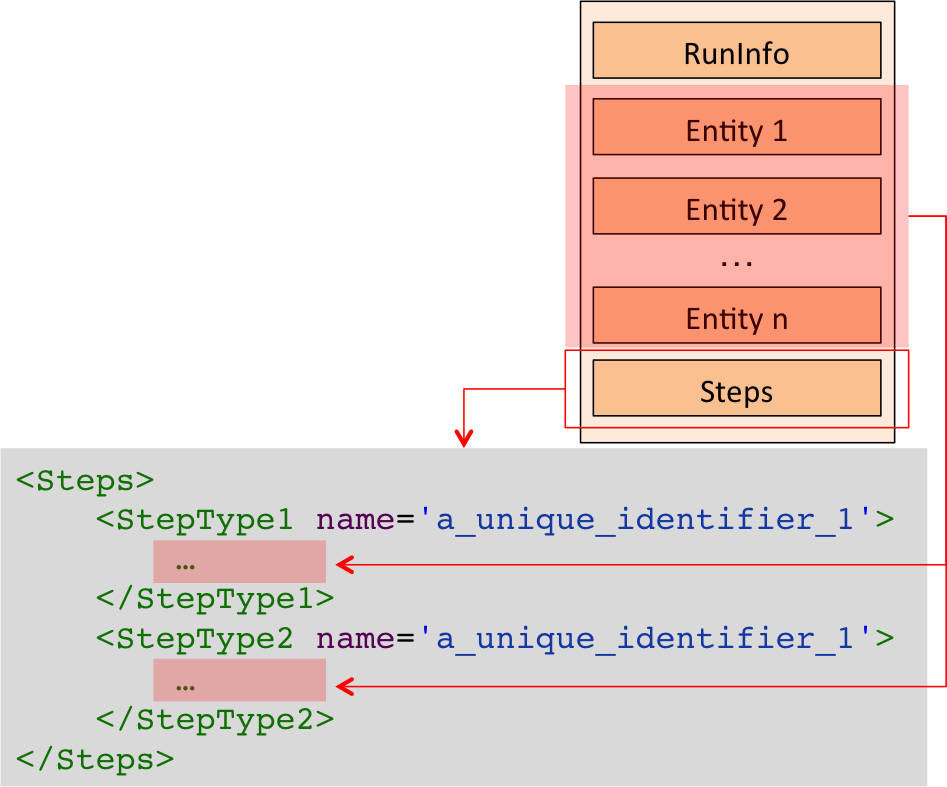
\includegraphics[scale=1]{pics/ExampleStepEntity.png}
  \caption{Example of the Steps \textbf{Entity}  and its connection in the input file.}
  \label{fig:ExampleStepEntity}
\end{figure}
  \item \textit{\textbf{Models}}:
  \\ The Models \textbf{Entity}  represents the projection from the input to the output space. Currently, RAVEN defines the
  following sub-categories:
      \begin{itemize}
       \item \textit{Code}, the sub-~\textbf{Entity} that represent the driven code, through external code interfaces (see~\cite{RAVENuserManual})
       \item  \textit{ExternalModel}, the sub-~\textbf{Entity} that represents a physical or mathematical model that is
       directly implemented by the user in a Python module
      \item \textit{ROM}, the sub-~\textbf{Entity} that represent the Reduced Order Model, interfaced with several algorithms
       \item \textit{PostProcessor}, the sub-~\textbf{Entity} that is used to perform action on data, such as computation of
       statistical moments, correlation matrices, etc.
      \end{itemize}
      The Model \textbf{Entity} can be seen as a transfer function between the input and output space.
  \item \textit{\textbf{Functions}}:
   \\ The Functions \textbf{Entity} is the container of all the user-defined functions, such as Goal Functions in adaptive
   sampling strategies, etc.
\end{itemize}
All these action-objects are combined together to create a peculiar analysis flow, which is specified
by the user in an additional \textbf{Entity} named \textit{\textbf{Steps}}. This \textbf{Entity} represents the core of the analysis, since it is the location where the multiple objects get finally linked in order to perform a combined action on a certain \textit{Model} (see Fig.~\ref{fig:ExampleStepEntity}). In order to perform this linking, each \textbf{Entity} defined in the Step needs to ``play'' a Role:
\begin{itemize}
  \item \textit{Input}
  \item \textit{Output}
  \item \textit{Model}
  \item \textit{Sampler}
  \item \textit{Function}
  \item \textit{ROM}
  \item \textit{SolutionExport}, the \textbf{Entity} that is used to export the solution of a \textit{Sampler}.
\end{itemize}
Currently, RAVEN supports 4 different types of \textit{\textbf{Steps}}:
\begin{itemize}
  \item \textit{SingleRun}, perform a single run of a model
  \item \textit{MultiRun}, perform multiple runs of a model
  \item \textit{RomTrainer}, perform the training of a Reduced Order Model (ROM)
  \item \textit{PostProcess}, post-process data or manipulate RAVEN entities
  \item \textit{IOStep}, step aimed to perform multiple actions:
  \begin{itemize}
    \item construct/update a Database from a DataObjects and vice-versa
    \item construct/update a Database or a DataObjects object from CSV files
    \item stream the content of a Database or a DataObjects out through an OutStream
    \item store/retrieve a ROM to/from an external File using Pickle module of Python
  \end{itemize}
\end{itemize}

\subsection{Raven Input Structure}
\label{sub:InputStructure}
The RAVEN code does not have a fixed calculation flow, since all of its basic
objects can be combined in order to create a user-defined calculation flow.
%
Thus, its input, eXtensible Markup Language (XML) format, is organized in different XML blocks, each with a
different functionality.
%
The main input blocks are as follows:
\begin{itemize}
  \item \textbf{\textless Simulation\textgreater}: The root node containing the
  entire input, all of
  the following blocks fit inside the \emph{Simulation} block.
  %
  \item \textbf{\textless RunInfo\textgreater}: Specifies the calculation
  settings (number of parallel simulations, etc.).
  %
  \item \textbf{\textless Files\textgreater}: Specifies the files to be
  used in the calculation.
  %
  \item \textbf{\textless Distributions\textgreater}: Defines distributions
  needed for describing parameters, etc.
  %
  \item \textbf{\textless Samplers\textgreater}: Sets up the strategies used for
  exploring an uncertain domain.
  %
  \item \textbf{\textless DataObjects\textgreater}: Specifies internal data objects
  used by RAVEN.
  %
  \item \textbf{\textless Databases\textgreater}: Lists the HDF5 databases used
  as input/output to a
  RAVEN run.
  %
  \item \textbf{\textless OutStreams\textgreater}: Visualization and
  Printing system block.
  %
  \item \textbf{\textless Models\textgreater}: Specifies codes, ROMs,
  post-processing analysis, etc.
  %
  \item \textbf{\textless Functions\textgreater}: Details interfaces to external
  user-defined functions and modules.
  %
  the user will be building and/or running.
  %
  \item \textbf{\textless Steps\textgreater}: Combines other blocks to detail a
  step in the RAVEN workflow including I/O and computations to be performed.
  %
\end{itemize}

Each of these blocks are explained in dedicated sections of the user manual ~\cite{RAVENuserManual}.
%
